\section{Проектирование и разработка средства оценки планируемой нагрузки на систему ввода-вывода PostgreSQL}

\subsection{Постановка требований к разрабатываемому средству}

Анализ существующих решений показывает, что ни один из подходов не ориентирован напрямую на предварительную оценку I/O-нагрузки без реального выполнения запросов. Поэтому к разрабатываемому средству предъявляются следующие требования:

\begin{itemize}
    \item \textbf{Прогнозирование без запуска нагрузки}: инструмент должен уметь оценивать предполагаемую нагрузку по метаданным базы данных и характеристикам планируемых запросов.
    \item \textbf{Поддержка типовых операций PostgreSQL}: необходимо учитывать особенности выполнения основных операций: вставка и выборка.
    \item \textbf{Оценка объема операций чтения и записи}: средство должно отдельно оценивать предполагаемые объемы чтения и записи данных.
    \item \textbf{Модульность и расширяемость}: архитектура решения должна позволять легко адаптировать его к новым версиям PostgreSQL и различным типам приложений.
    \item \textbf{Простота использования}: инструмент должен быть доступен для использования специалистами без глубокого знания внутренней архитектуры PostgreSQL.
\end{itemize}


\subsection{Разработка программного средства}



\subsubsection{Выбор инструментов и технологий}

Выбор инструментов и технологий, использованных при разработке программного средства, был обусловлен как специфическими требованиями предметной области (прогнозирование нагрузки на СУБД PostgreSQL), так и общими соображениями масштабируемости, воспроизводимости и автоматизации. В данном подразделе приведён обоснованный выбор программных средств, языков программирования, форматов представления данных и средств автоматизации.

\paragraph{Язык программирования Python}

В качестве основного языка реализации был выбран Python. Основные причины выбора следующие:

\begin{itemize}
  \item \textbf{Высокий уровень абстракции}. Python предоставляет удобные средства для работы со строками, файлами, регулярными выражениями и структурами данных, что особенно актуально при анализе SQL-описаний (DDL) и конфигурационных файлов.
  \item \textbf{Богатая экосистема}. Используемые стандартные библиотеки (\texttt{yaml}, \texttt{re}, \texttt{math}, \texttt{argparse}) полностью покрывают потребности проекта без необходимости в дополнительных зависимостях.
  \item \textbf{Удобство для прототипирования}. Язык позволяет быстро разрабатывать и отлаживать модули, что особенно важно на этапе научных экспериментов и итеративной разработки.
\end{itemize}

\paragraph{Формат конфигурации: YAML}

Для задания входных параметров алгоритма был выбран формат YAML по следующим причинам:

\begin{itemize}
  \item \textbf{Читаемость}. YAML близок к естественному синтаксису и легко воспринимается человеком, что снижает порог входа для конечных пользователей и разработчиков.
  \item \textbf{Иерархичность}. Формат удобно отражает вложенные структуры, такие как описание нескольких таблиц с DDL, параметры нагрузки и конфигурацию окружения.
  \item \textbf{Совместимость с Python}. Модуль \texttt{PyYAML} обеспечивает простую загрузку данных YAML в структуры Python (словарь, список и т.д.).
\end{itemize}

\paragraph{Shell-скрипты и автоматизация}

Для автоматизации запуска программного средства и обработки множественных конфигурационных файлов использовались скрипты командной оболочки Bash. Их функции включают:

\begin{itemize}
  \item \textbf{Циклический запуск анализа} по множеству входных YAML-файлов.
  \item \textbf{Агрегация и вывод результатов} в удобном табличном формате.
  \item \textbf{Интеграция с системой CI/CD}, в частности, в рамках GitHub Actions.
\end{itemize}

Использование Bash позволяет не привязывать обработку к конкретной ОС, поскольку все компоненты являются кроссплатформенными и не требуют сторонних зависимостей.

\paragraph{GitHub Actions}

Система GitHub Actions используется для автоматизации тестирования и анализа кода в момент каждого коммита или пулл-запроса. Преимущества выбора данной технологии:

\begin{itemize}
  \item \textbf{Автоматический запуск проверок} при каждом изменении кода.
  \item \textbf{Гарантия воспроизводимости} за счёт запуска в изолированном контейнерном окружении.
  \item \textbf{Интеграция с репозиторием} без необходимости использования внешних CI-серверов.
\end{itemize}

В рамках проекта реализован отдельный workflow-файл, который инициирует запуск Bash-скрипта, передаёт необходимые параметры и сохраняет результаты анализа.

\paragraph{Пользовательский web-интерфейс: React + JavaScript}

Для повышения удобства взаимодействия с программным средством и расширения целевой аудитории был разработан современный web-интерфейс на основе библиотеки React. Данный компонент реализует пользовательскую форму для задания входных данных: структуры таблиц, конфигурации PostgreSQL, параметров нагрузки и запросов.

Основные причины выбора React:

\begin{itemize} \item \textbf{Динамичность интерфейса}. React обеспечивает реактивное обновление состояния и рендеринг формы в зависимости от пользовательских действий, что критически важно в задачах интерактивного конфигурирования параметров. \item \textbf{Поддержка сложных форм}. Библиотека позволяет удобно реализовывать динамические добавления и редактирование таблиц, параметров, выводить подсказки и валидировать вводимые значения на лету. \item \textbf{Развитая экосистема}. Использование сторонних библиотек (например, Papaparse для обработки CSV с подсказками по конфигурации) существенно упрощает реализацию и расширение функционала. \item \textbf{Кроссплатформенность и доступность}. React-приложение легко развёртывается как отдельный SPA, интегрируется с серверной частью через REST API или может разворачиваться как statically-served сайт в любом окружении. \item \textbf{Масштабируемость}. Архитектура React позволяет в будущем легко интегрировать новые функции: графики (например, через Plotly), автоматическую проверку корректности вводимых DDL или расширенные формы для разных сценариев нагрузки. \end{itemize}

Базовый функционал разработанного интерфейса включает:

\begin{itemize} \item Формирование и редактирование списка таблиц с интуитивным вводом DDL и числа строк; \item Автоматизированный подбор и изменение параметров конфигурации PostgreSQL с поясняющими подсказками, загружаемыми из справочных данных; \item Ввод тестового SQL-запроса и параметра нагрузки (RPS); \item Поддержку вложенных, типизированных и связанных параметров (разделение числовых значений и единиц измерения, on/off-переключатели, списки и т.д.). \end{itemize}

Реализация приложения на React позволила обеспечить современный UX и повысить скорость конфигурирования, а также снизить требования к технической подготовке конечного пользователя, по сравнению с ручным редактированием YAML-файлов.

\paragraph{Вывод}

Таким образом, совокупность выбранных технологий обеспечивает гибкость, воспроизводимость, автоматизируемость и пользовательскую доступность разработанного программного средства. При этом архитектура построена таким образом, что допускает расширение функциональности и адаптацию под иные СУБД или сценарии нагрузки в будущем.




\subsubsection{Описание алгоритма прогнозирования}

Разработанный алгоритм предназначен для прогнозирования объёма дискового пространства, необходимого для хранения пользовательских данных в системе управления базами данных PostgreSQL, а также для предварительной оценки предполагаемой нагрузки (в терминах RPS --- запросов в секунду) на отдельные компоненты файловой подсистемы. Алгоритм реализован на языке программирования Python и ориентирован на статический анализ конфигурационных данных и DDL-описаний таблиц.

\vspace{0.5em}
\noindent
Основными этапами работы алгоритма являются:

\begin{enumerate}
    \item \textbf{Извлечение структурной информации из DDL-описания.} 
    С использованием регулярных выражений производится синтаксический разбор SQL-команды создания таблицы (\texttt{CREATE TABLE}). Алгоритм выделяет список столбцов с соответствующими типами данных, а также определяет тип индекса, если он указан явно (например, \texttt{BTREE}, \texttt{GIN}, \texttt{HASH} и др.). Предусмотрена обработка ключевых слов, указывающих на составные ключи и особенности индексирования.

    \item \textbf{Оценка объёма хранения одной строки таблицы.}
    Для каждого столбца производится оценка объёма занимаемой памяти в байтах. В рамках текущей реализации реализована эвристическая схема оценки:
    \begin{itemize}
        \item целочисленные типы (\texttt{INT}, \texttt{BIGINT}) оцениваются в 4 байта;
        \item типы \texttt{NUMERIC} --- в 16 байт;
        \item типы временных меток (\texttt{TIMESTAMP}) --- в 8 байт;
        \item символьные типы (\texttt{CHAR(n)}) --- в $n$ байт;
        \item переменные по длине типы, такие как \texttt{TEXT} и \texttt{JSON}, принимаются равными 2000 и 3000 байт соответственно.
    \end{itemize}
    Кроме того, добавляется фиксированный системный оверхед в 24 байта на каждую строку.

    \item \textbf{Учет механизма TOAST.}
    В случае, если совокупный размер строки превышает установленный порог (в PostgreSQL это обычно 2000 байт), предполагается использование механизма TOAST (The Oversized-Attribute Storage Technique). В таком случае создаётся отдельная сущность хранения, и её объём также включается в итоговую оценку. Размер строки в основной таблице после вынесения больших атрибутов оценивается условно в 50 байт.

    \item \textbf{Расчет плотности хранения и общего количества страниц.}
    Учитывается размер страницы PostgreSQL (\texttt{PAGE\_SIZE} = 8192 байт) и коэффициент заполнения страницы (\texttt{FILL\_FACTOR} = 0{,}85). На основе рассчитанного размера строки определяется количество строк на одной странице и далее --- общее число страниц, необходимое для хранения всех строк таблицы.

    \item \textbf{Формирование структуры хранения.}
    Для каждой таблицы формируется совокупность логических файлов, соответствующих различным компонентам системы хранения PostgreSQL:
    \begin{itemize}
        \item основной heap-файл таблицы;
        \item TOAST-таблица (при необходимости);
        \item индексный файл (в зависимости от типа индекса);
        \item карты свободного пространства (FSM --- Free Space Map);
        \item карты видимости (VM --- Visibility Map).
    \end{itemize}
    Для каждого из указанных компонентов вычисляется примерный размер в байтах и фиксируется предполагаемый тип доступа (например, ``Heap access (join read)'', ``Index (btree)'', ``TOAST read/write'' и др.).

    \item \textbf{Оценка нагрузки (RPS).}
    В конфигурационном файле YAML указывается SQL-запрос, который будет исполняться в рамках моделируемой нагрузки. Алгоритм выделяет из запроса имена задействованных таблиц (анализируя конструкции \texttt{FROM} и \texttt{JOIN}) и помечает соответствующие таблицы как ``активные''. Только активным таблицам присваивается значение RPS, указанное в конфигурации. Для неактивных таблиц нагрузка считается нулевой.

    \item \textbf{Вывод и визуализация результатов.}
    На выходе алгоритм формирует таблицу, содержащую информацию по каждому логическому файлу: имя, размер в килобайтах, значение RPS и характер доступа. Эта информация может быть выведена как в консольном интерфейсе, так и, при интеграции с веб-приложением, в виде интерактивной HTML-таблицы.
\end{enumerate}

\vspace{0.5em}
\noindent
Таким образом, предложенный алгоритм позволяет без запуска СУБД и исполнения реальных SQL-запросов получить оценку распределения нагрузки на файловую подсистему PostgreSQL. Это делает его полезным инструментом как для предварительного анализа схемы данных, так и для целей тестирования, анализа производительности и оптимизации структуры хранения.



\subsubsection{Формат входных данных основного алгоритма}

Входные данные для алгоритма прогнозирования нагрузки на диск представляются в виде конфигурационного файла в формате YAML. Данный файл отражает как логическую структуру обрабатываемых данных, так и параметры выполнения запроса, характеристики окружения и конфигурационные настройки PostgreSQL, влияющие на поведение подсистемы хранения. Формат входного файла структурирован и предназначен как для автоматической обработки, так и для удобства ручного редактирования.

Файл включает четыре логических блока: \texttt{tables}, \texttt{load\_generator}, \texttt{postgresql\_config}, \texttt{environment}.

\paragraph{Блок \texttt{tables}}

Раздел \texttt{tables} представляет собой список таблиц, каждая из которых описывается следующими параметрами:

\begin{itemize}
  \item \texttt{name}~--- строка, задающая уникальное имя таблицы.
  \item \texttt{ddl}~--- SQL-выражение \texttt{CREATE TABLE}, задающее схему таблицы (с типами столбцов, индексами, ключами).
  \item \texttt{row\_count}~--- предполагаемое количество строк в таблице, необходимое для оценки объёма хранимых данных и числа используемых страниц.
\end{itemize}

Алгоритм парсит DDL-описание таблиц для определения размера строк, необходимости TOAST-хранилища, типа индексной структуры и особенностей хранения массивов и JSONB-типов.

\paragraph{Блок \texttt{load\_generator}}

Данный блок описывает модель генерируемой нагрузки на базу данных, имитируя поведение прикладного уровня:

\begin{itemize}
  \item \texttt{query}~--- SQL-запрос, на основе которого осуществляется прогнозирование интенсивности обращений к таблицам. Из запроса извлекаются участвующие в соединениях таблицы и предполагаемая направленность доступа (например, только чтение).
  \item \texttt{rps} (requests per second)~--- оценка числа запросов в секунду, поступающих к указанному SQL-запросу. Данный параметр масштабирует итоговую нагрузку, распределяя её между таблицами и индексами, участвующими в запросе.
\end{itemize}

\paragraph{Блок \texttt{postgresql\_config}}

Конфигурация PostgreSQL включает все основные параметры, оказывающие влияние на поведение подсистемы хранения данных. Среди них:

\begin{itemize}
  \item \textbf{Буферизация и кэширование}:
    \begin{itemize}
      \item \texttt{shared\_buffers}~--- объём оперативной памяти, зарезервированный под буферы PostgreSQL.
      \item \texttt{effective\_cache\_size}~--- оценка размера файлового кэша, доступного PostgreSQL со стороны ОС.
      \item \texttt{work\_mem}, \texttt{maintenance\_work\_mem}~--- лимиты памяти на операции сортировки и создания индексов.
    \end{itemize}

  \item \textbf{Конфигурация WAL и контрольных точек (checkpoints)}:
    \begin{itemize}
      \item \texttt{wal\_buffers}, \texttt{max\_wal\_size}, \texttt{min\_wal\_size}, \texttt{wal\_compression}~--- параметры объёма и сжатия журналов WAL.
      \item \texttt{checkpoint\_timeout}, \texttt{checkpoint\_completion\_target}~--- параметры частоты и длительности контрольных точек.
      \item \texttt{fsync}, \texttt{synchronous\_commit}~--- параметры, определяющие, требуется ли жёсткая синхронизация данных на диск при коммите.
    \end{itemize}

  \item \textbf{Автовакуум и фоновая активность}:
    \begin{itemize}
      \item \texttt{autovacuum}, \texttt{autovacuum\_max\_workers}, \texttt{autovacuum\_naptime}~--- параметры частоты и параллелизма фоновой очистки таблиц.
      \item \texttt{autovacuum\_vacuum\_cost\_limit}, \texttt{autovacuum\_vacuum\_cost\_delay}~--- параметры скорости фонового VACUUM.
    \end{itemize}

  \item \textbf{Оценки стоимости операций}:
    \begin{itemize}
      \item \texttt{random\_page\_cost}, \texttt{seq\_page\_cost}~--- логические параметры, отражающие относительную стоимость случайного и последовательного чтения страниц. Используются в планировщике запросов и влияют на стратегию доступа к данным.
    \end{itemize}

  \item \textbf{Прочие параметры}:
    \begin{itemize}
      \item \texttt{wal\_level}~--- уровень детализации WAL, определяющий объём логирования и, соответственно, нагрузку на диск.
      \item \texttt{wal\_writer\_delay}~--- задержка между фоновыми сбросами WAL на диск.
      \item \texttt{temp\_buffers}~--- объём памяти, выделяемый на временные таблицы, участвующие в запросах.
    \end{itemize}
\end{itemize}

\paragraph{Блок \texttt{environment}}

Описывает характеристики вычислительного окружения, на котором предполагается выполнение анализа:

\begin{itemize}
  \item \texttt{cpu\_cores}~--- количество доступных процессорных ядер.
  \item \texttt{ram\_gb}~--- общий объём оперативной памяти в гигабайтах.
  \item \texttt{storage\_type}~--- тип дисковой подсистемы (например, \texttt{ssd}, \texttt{hdd}, \texttt{nvme}).
  \item \texttt{os\_cache\_enabled}~--- булев флаг, указывающий, доступен ли файловый кэш со стороны ОС.
\end{itemize}

\paragraph{Вывод}

Предложенный формат конфигурационного файла обеспечивает достаточную полноту и выразительность для оценки поведения системы хранения PostgreSQL при различных сценариях нагрузки. YAML-представление обеспечивает читаемость, расширяемость и лёгкую интеграцию с автоматическими средствами анализа и визуализации.



\insertlisting{Содержимое файла \texttt{example1.yaml}}{code/example1.yaml}


\subsubsection{Формат выходных данных алгоритма предсказания нагрузки на систему ввода-вывода}

Выходные данные алгоритма предсказания нагрузки на подсистему ввода-вывода представлены в формате YAML, отражающем структурированное описание файловых компонентов системы управления базами данных PostgreSQL, участвующих в операциях хранения и извлечения данных. Формат включает параметры физического хранения, объёмы, характер обращений и модель оценки производительности в условиях различной эффективности кэширования.

Каждый логический файл базы данных описывается в отдельной структуре с обязательным указанием следующих атрибутов:
\begin{itemize}
    \item \texttt{name} --- абсолютный путь к файлу в файловой системе PostgreSQL;
    \item \texttt{type} --- тип файла: основной (heap), вспомогательный (TOAST), индексный (btree\_index), карта свободного пространства (fsm);
    \item \texttt{estimated\_size\_mb} --- предполагаемый объём файла в мегабайтах;
    \item \texttt{access\_pattern} --- описание характера обращений к файлу, включая совокупное количество операций (\texttt{total\_operations}) и сценарии обращения при различных коэффициентах попадания в кэш;
    \item \texttt{io\_scenarios} --- набор параметров, описывающих производительность при заданной доле кэшированных операций (\texttt{cache\_hit\_ratio}). Для каждого сценария указываются:
    \begin{itemize}
        \item \texttt{read\_ops} --- количество операций чтения, направленных непосредственно к устройствам хранения;
        \item \texttt{write\_ops} --- количество операций записи;
        \item \texttt{read\_throughput\_mb\_s} --- оценка пропускной способности по чтению (в мегабайтах в секунду);
        \item \texttt{write\_throughput\_mb\_s} --- оценка пропускной способности по записи.
    \end{itemize}
\end{itemize}

Алгоритм учитывает четыре основные модели кэширования:
\begin{enumerate}
    \item $0\%$ попаданий в кэш (все обращения направлены к физическому диску);
    \item $25\%$ попаданий в кэш;
    \item $50\%$ попаданий в кэш;
    \item диапазон $50\text{--}80\%$ кэш-хитов, имитирующий реальное поведение при высокоэффективных буферных пулах.
\end{enumerate}

Дополнительно структура YAML содержит секцию \texttt{metadata}, в которой указываются единицы измерения параметров и поясняющие примечания.

Пример соответствующего YAML-файла приведён ниже:
\begin{quote}
\footnotesize
\begin{verbatim}
postgres_disk_io_prediction:
  database: my_database
  tablespace: pg_default
  files:
    - name: base/16384/12345
      type: heap
      estimated_size_mb: 2048
      access_pattern:
        total_operations: 500000
        io_scenarios:
          - cache_hit_ratio: 0.0
            read_ops: 300000
            write_ops: 200000
            read_throughput_mb_s: 80
            write_throughput_mb_s: 40
          ...
metadata:
  units:
    size: MB
    throughput: MB/s
    operations: iops (read/write)
  notes:
    - "cache_hit_ratio refers to percentage of data read from memory (not disk)"
    - "Estimated throughput is approximate and hardware dependent"
\end{verbatim}
\end{quote}

Данный формат обеспечивает пригодность для последующего анализа, визуализации и генерации нагрузочного тестирования в системах моделирования ввода-вывода или автоматизированных средствах администрирования СУБД PostgreSQL.




\subsection{Реализация web-интерфейса}
\subsubsection{Основные требования к web-интерфейсу}

Одной из главных задач при разработке средства оценки пла\-ни\-руемой наг\-руз\-ки на систему ввода-вывода СУБД PostgreSQL является создание интуитивно понятного и функционального web-интерфейса, обеспечивающего пользователю удобный ввод параметров моделирования и получение рекомендаций по настройке среды. Интерфейс должен позволять пользователю задавать параметры конфигурации СУБД PostgreSQL, а также характеристики используемых таблиц и SQL-запросов, что необходимо для построения корректной модели нагрузки.


\subsubsection{Выбор инструментов реализации}

В качестве основы для реализации web-интерфейса был выбран фреймворк React, известный своей модульностью, высоким уровнем абстракции и поддержкой современных парадигм разработки SPA (Single-page Application). Для удобной работы с CSV-файлами использовалась библиотека \texttt{papaparse}, посредством которой реализована подгрузка текстовых подсказок (hints) по настройкам из внешнего файла с рекомендациями. Также применялись инструменты для унификации и стилизации пользовательского интерфейса (CSS, Tailwind).

\subsubsection{Архитектура и компоненты интерфейса}

Разработанный web-интерфейс логически состоит из следующих основных модулей:
\begin{itemize}
    \item форма для ввода перечня таблиц, хранящихся в СУБД, их определяющих конструкций (DDL) и приблизительных размеров (количества строк);
    \item панель настройки параметров конфигурации PostgreSQL с разделением полей по единицам измерения (байты, время, бинарные параметры);
    \item секция для задания SQL-запроса и интенсивности работы (RPS --- запросы в секунду).
\end{itemize}

Структура интерфейса разбита на секции для повышения читаемости и модульности. Взаимодействие между компонентами осуществляется посредством \emph{состояний} (React Hooks), что обеспечивает мгновенное обновление данных при изменениях, совершённых пользователем.

На рисунке~\ref{img:interface} изображён внешний вид основной страницы web-интерфейса.

\begin{figure}[H]
    \centering
    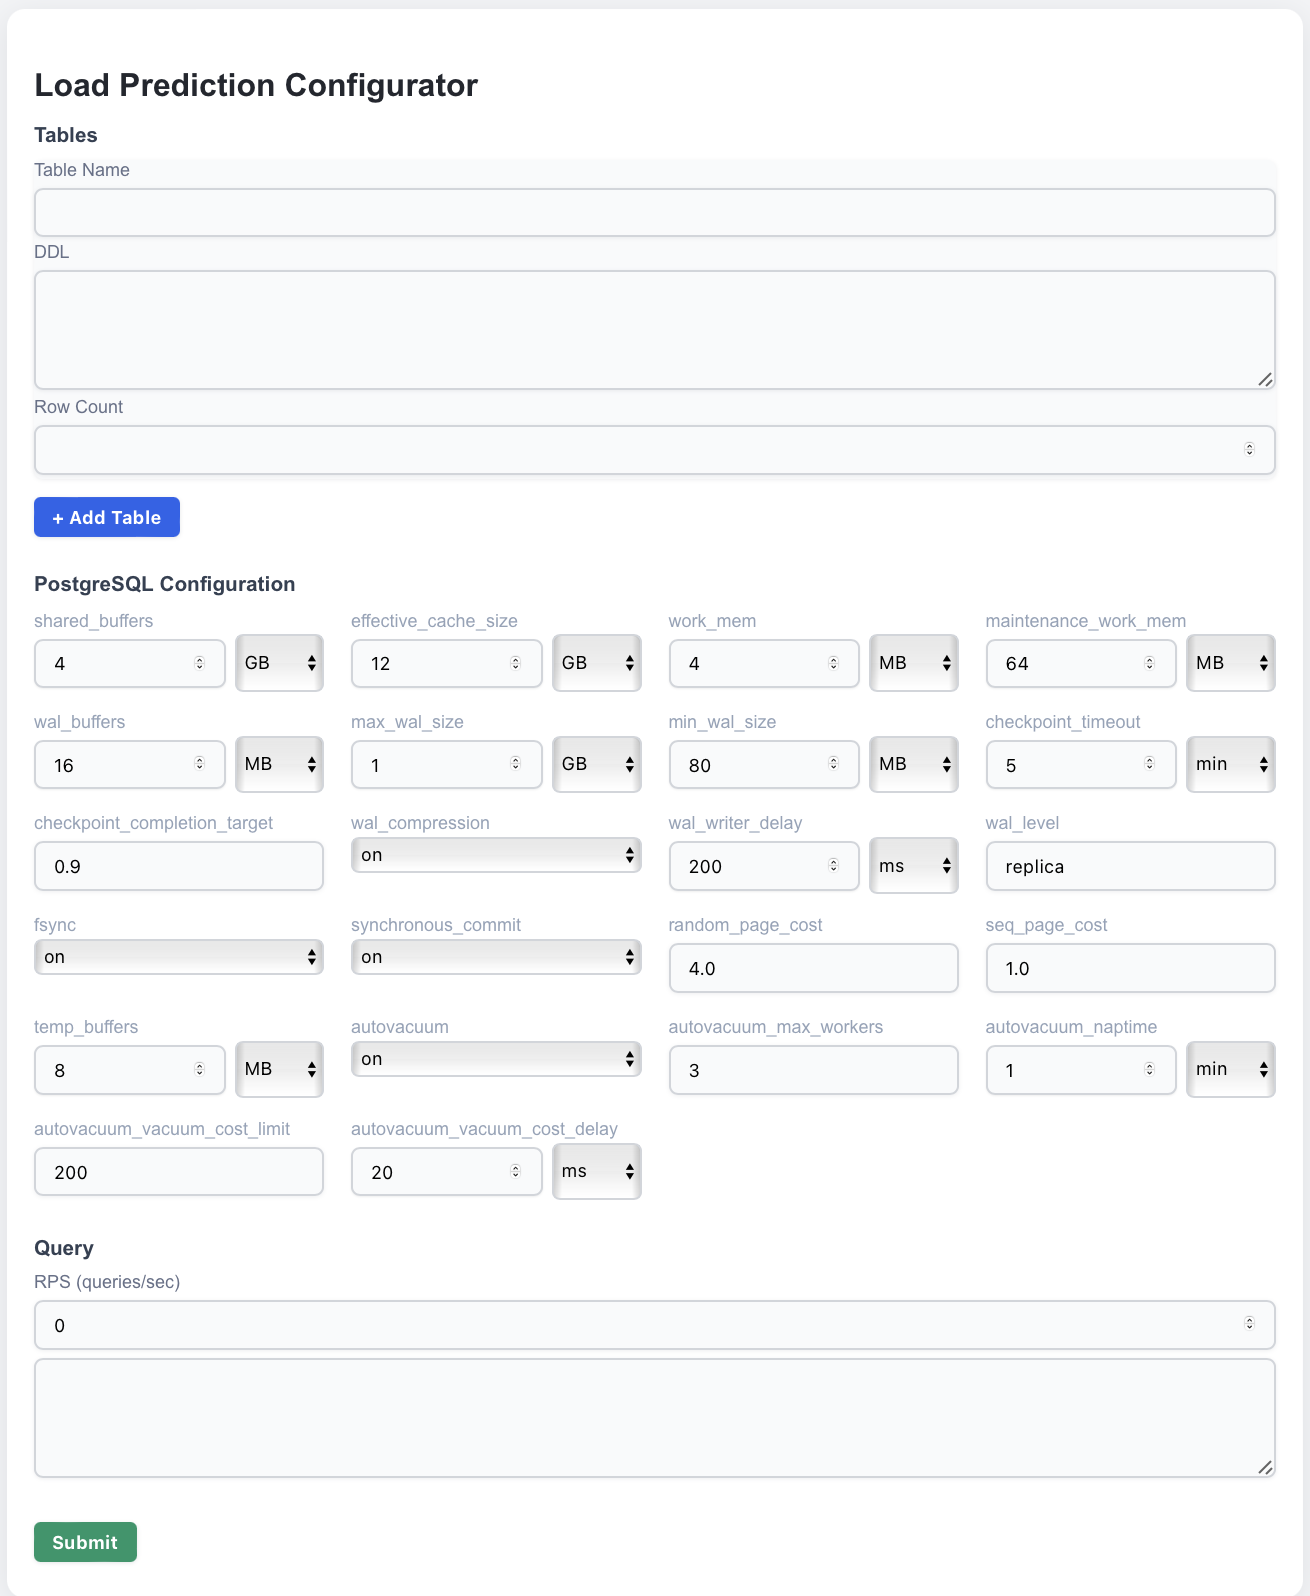
\includegraphics[width=0.95\textwidth]{images/interface.png}
    \caption{Внешний вид реализованного web-интерфейса средства оценки нагрузки.}
    \label{img:interface}
\end{figure}

\subsubsection{Ввод информации о таблицах}

Пользователь может добавить неограниченное количество схем таблиц, каждая из которых описывается тройкой параметров:
\begin{itemize}
    \item название таблицы (\emph{Table Name});
    \item определяющая конструкция DDL (\emph{DDL}), указывается в формате SQL;
    \item предполагаемое количество строк (\emph{Row Count}), что критически важно для моделирования нагрузки.
\end{itemize}
Для добавления очередной таблицы реализована кнопка \emph{``+ Add Table''}. Изменения применяются немедленно, значения инкапсулируются в соответствующем состоянии.

\subsubsection{Панель настройки параметров PostgreSQL}

Особое внимание уделяется корректной обработке различных типов параметров конфигурации СУБД:
\begin{itemize}
    \item параметры включения/выключения (\emph{on/off}) --- выводятся в виде выпадающих списков;
    \item временные и объёмные (байтовые) параметры разбиты на числовую часть и единицу измерения, что минимизирует ошибки пользователя;
    \item остальные параметры визуализируются в виде текстовых полей.
\end{itemize}

Каждое поле сопровождается интерактивной подсказкой, расположенной под ним, если для данного ключа имеется поясняющий текст в подгруженном \texttt{postgres\_config\_hints.csv}. Это способствует правильному выбору пользователем подходящих значений.

\subsubsection{Ввод SQL-запроса и интенсивности работы}

В специальной секции пользователь вводит синтаксис моделируемого SQL-запроса (или его шаблон), а также задаёт интенсивность нагрузки (RPS, запросы в секунду). Эти данные необходимы для последующего прогноза нагрузки на систему ввода-вывода.

\subsubsection{Валидация и обработка введённых данных}

Реализация контролирует тип полей (текст, число, выпадающий список), диапазон вводимых значений, корректность комбинации числа и единицы измерения. Вся логика обработки ввода инкапсулирована в компоненте приложения, состояние синхронизируется с действиями пользователя.

\subsubsection{Взаимодействие с серверной частью}

После нажатия кнопки \emph{Submit} собранные параметры отправляются на сервер для последующей обработки. Серверная логика, реализованная отдельно, использует полученные данные для анализа и моделирования I/O-нагрузки СУБД PostgreSQL.

\subsubsection{Резюме по реализации интерфейса}

Итоговая реализация web-интерфейса позволяет гибко задать все существенные параметры, необходимые для моделирования нагрузки и последующего анализа. Структура интерфейса обеспечивает как простоту начального освоения, так и расширяемость. Выбранные технологические решения и разделение логики на отдельные компоненты обеспечивают независимость модулей, устойчивость к ошибкам и возможность масштабирования при развитии проекта.


\subsubsection{Автоматизация запуска с помощью Bash и интеграция с GitHub Actions}

Автоматизация рутинных задач является важной частью современного программирования, позволяя разработчикам сосредоточиться на решении более сложных и творческих задач. В данном разделе рассмотрим процесс автоматизации запуска скрипта с использованием Bash и его интеграцию в процесс CI/CD посредством GitHub Actions.

\textbf{Структура проекта}

Проект структурирован таким образом, чтобы обеспечить простую навигацию и легкость понимания. Корневая директория содержит основной скрипт запуска, \texttt{run-examples.py}, который представляет собой Bash-скрипт для управления виртуальным окружением Python и выполнения анализатора. В корневой директории также находится файл зависимостей \texttt{requirements.txt}, а примеры, предназначенные для анализа, располагаются в подкаталогах, соответствующих шаблону \texttt{examples/example*/\ *.yaml}.

 
\begin{figure}[H]
    \centering
    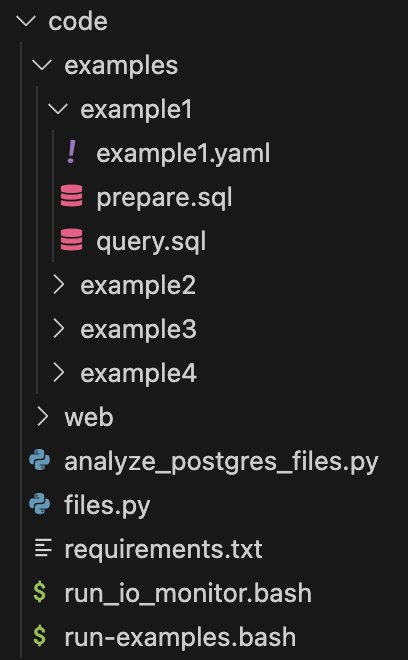
\includegraphics[width=0.4\textwidth]{images/project-structure.png}
    \caption{Структура файлов в проекте.}
    \label{img:project-structure}
\end{figure}

\textbf{Описание \texttt{run-examples.py}}

Скрипт \texttt{run-examples.py} выполняет несколько ключевых задач:

Создание виртуального окружения: Если директория \texttt{venv} отсутствует, создается новое виртуальное окружение.
Активация окружения: Виртуальное окружение активируется посредством команды \texttt{source}.
Обновление pip: Перед установкой зависимостей обновляется пакетный менеджер \texttt{pip}.
Установка зависимостей: Зависимости устанавливаются из файла \texttt{requirements.txt}, если он доступен.
Анализ YAML-файлов: Скрипт последовательно проходит по каждому YAML-файлу в директории примеров и запускает анализатор \texttt{analyze\_postgres\_files.py}.
Деактивация окружения: Завершает работу, деактивируя виртуальное окружение.
Каждый шаг содержит проверку на наличие ошибок, что позволяет скрипту надёжно обрабатывать исключительные ситуации, делая его более стабильным и надежным.

\textbf{Интеграция с GitHub Actions}

GitHub Actions предоставляет мощные инструменты для автоматизации рабочих процессов. Интеграция Bash-скрипта в процесс CI/CD с помощью GitHub Actions позволяет запускать анализатор автоматически при каждом коммите. Ниже приведен пример конфигурации рабочего процесса:

\begin{center}
\textbf{Листинг 1} --- Содержимое файла \texttt{actions.yaml}
\end{center}

\lstinputlisting[language=yaml]{code/actions.yaml}


\subsubsection{Резюме по реализации программного средства}

В данной работе было реализовано программное средство для оценки объёмов и интенсивности обращения к дисковым структурам в системе управления базами данных PostgreSQL на основе анализа схемы данных, предполагаемой нагрузки и параметров окружения.

Разработка выполнена с применением интерпретируемого языка Python, что обеспечило гибкость, расширяемость и удобство интеграции с другими компонентами инфраструктуры. Основной модуль программы реализует алгоритм прогнозирования, который производит анализ описания таблиц в формате DDL, рассчитывает размер строк, распределение данных по страницам и необходимость использования механизмов TOAST. Также учитываются вторичные структуры хранения, включая индексы различных типов (btree, GIN, GiST и др.), карты свободного и видимого пространства (FSM и VM), а также влияние параметров буферизации.

Входные данные подаются в формате YAML, что позволяет обеспечить наглядную и декларативную спецификацию характеристик базы данных и параметров нагрузки. Алгоритм автоматически интерпретирует SQL-запрос, извлекая перечень таблиц, участвующих в операциях соединения, что критически важно для корректного распределения запросов (RPS) между различными структурами хранения.

В рамках реализации обеспечена автоматизация процессов запуска: реализованы вспомогательные Bash-скрипты, позволяющие последовательно обрабатывать набор тестовых конфигураций. Интеграция с системой непрерывной интеграции GitHub Actions обеспечивает повторяемость и прозрачность выполнения тестов при каждом изменении кода.

Дополнительно был реализован прототип web-интерфейса, предоставляющий пользователю возможность загружать конфигурационные файлы, запускать анализ и визуализировать результаты прогнозирования в удобной форме. Это делает разработанное средство пригодным как для целей экспериментальной оценки, так и для использования в образовательных и консалтинговых задачах по проектированию архитектуры СУБД.

Таким образом, полученное программное решение представляет собой законченный и воспроизводимый инструмент, позволяющий на основе декларативного описания схемы и нагрузки предварительно оценивать нагрузку на подсистему хранения данных PostgreSQL без необходимости реального развёртывания полноценных нагрузочных тестов.

